\chapter{The Campaign}

\subsection{Tempestas}

At the start of the campaign, the DM needs to decide on a reason for the characters to be coming into Tempestas. This can be any good reason that fits with the player backstories or one from the following list. Tempestas is a large city with many things to do. The city will start closed off due to the impending threat of the Celestials attacking nearby cities. From Tempestas, the players can be lead to Aurushire. Different reasons can lead them to Aurushire such as the sport of the jungles or the search for the Trinity stones. Little do they know that the Trinity stones are the key to obtaining the San'graal to defeat the Celestials.

The players can start out in Tempestas either by living there, being in the prison there, or arriving there by spice trade (depending on the character backgrounds). While in Tempestas, they can encounter a few important characters such as Dastan and the fortuneteller. While in Tempestas, a Prior of the Celestas will also arrive and start his preaching. 

\subsection{Journey to Aurushire}

\begin{commentbox}{Journey to Aurushire}
	\begin{description}
		\item[For the Stones] Legend has it that there are rare and priceless artifacts hidden on Statu. It is possible that the player could be hunting the legends which have lead them to Aurushire.
		\item[The Rare Sport of Rem Silva] It is possible that the rare game in Rem Silva was spoken of and the players could be after the rare sport that resides in this area.
	\end{description}
\end{commentbox}

After leaving Tempestas by boat (If the party gets to this), they will have some rest time on the ship they are on. The tripe is generally only about a day or two away from Statu, however the party will encounter rough weather. The rough weather will turn into a massive storm in which the ship will be knocked around, back and forth. The party will be knocked unconscious and awake on the coast due east on Aurushire (without knowing of course) with only the players that are in their party and none of the NPCs from the ship. The cost will have rock and cliff faces to their east, and rough forest and mountains (appears unclimbable) to the North. Their only option is the the west. The west will lead into the Convallis swamp and marsh area's which is directly east of the Naga encampments. A thick fog will appear as they are traveling and they will need to navigate through rough swampy regions where they will encounter serpent Naga forces and some magical beasts like a witch hunter. After navigating through this region, the party will arrive and Aurushire, battered and beaten.

After arriving at Aurushire, there are many options for the players. There is an Inn (Prancing Pony Inn), where they can get rest. There are farms, where the players could potentially work. There are the mines, run by a Pandaren brother, where players could also work. There is a blacksmith, which is run by one of the three Pandaren brothers. There is the brewery/tavern, which is run by another Pandaren brother for players to socialize, learn, and relax. There is also Bob's Guns. Bob is a strange fella who claims is he from a more modern time. He has things that you cannot find anywhere else. To the northeast there is an old witch named Nev\'{a}r. To the northwest a wizard named Baba. Together the two are sometimes referred to as the Ying-Yang. For one appears good, and one appears the opposite. Though this name comes from the matter of looks, and not actions. 

\subsection{Baba}

Baba is a powerful wizard who has spent many lifetimes studying the flow of time and impacts of the time stone on the surrounding regions. Baba can be found throughout the time line as different versions of herself. At one point she found a way to manipulate the temporal and spacial fluctuations throughout the region to create copies of herself in different space-times. From this, there are Baba's hidden throughout the time line all living as separate entities. 

Baba's role can be whatever the DM likes. She was intended to persuade the users to seek the trinity stones. Along with this, Baba knows the powers and trickery of the stones and would not believe the party is ready no matter how experienced. Because of this, she can teleport them to various locations for trials such as the halls of no end \ref{maps} or the various surrounding regions. 

\begin{center}
	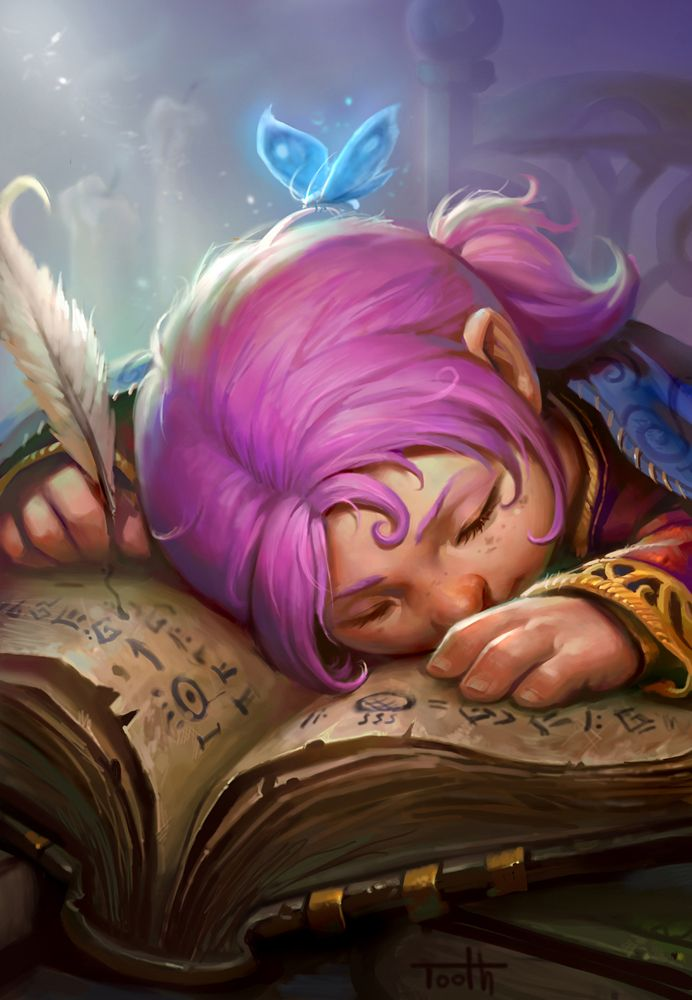
\includegraphics[width=0.5\linewidth]{img/baba.jpg}
\end{center}

\begin{monsterbox}{Baba}
	\begin{hangingpar}
		\textit{Gnome Wizard, Neutral Good}
	\end{hangingpar}
	\dndline%
	\basics[%
	armorclass = 24,
	hitpoints  = 302,
	speed      = 60 ft
	]
	\dndline%
	\stats[
	STR = \stat{8}, % This stat command will autocomplete the modifier for you
	DEX = \stat{16},
	CON = \stat{19},
	INT = \stat{20},
	WIS = \stat{20},
	CHA = \stat{19}
	]
	\dndline%
	\details[%
	% If you want to use commas in these sections, enclose the
	% description in braces.
	% I'm so sorry.
	languages = {Common, Elvish, Dwarvish, Gnomish, Halfling, Orc, Pandaren, Celestial, Draconic, Primordial},
	challenge = 20
	]
	\dndline%
	\begin{monsteraction}[Telekinesis]
		The ability to move objects with your mind. There is no limitation to how the objects can be moved if the objects belong to you.
	\end{monsteraction}	
	\begin{monsteraction}[Cerebral Warp]
		You can place humanoids into a deep illusion that seems completely real. The subjects cannot be harmed in the illusion.
	\end{monsteraction}	
	\begin{monsteraction}[Illusionary Presence]
		When you are near others, you feel to them to be in multiple places at once. If struck by a melee attack, you can relocate to an alternate location within 10 feet.
	\end{monsteraction}
	\begin{monsteraction}[Precision Striking]
		When you attack, you can choose hwo much damage to deal up to the amount shown on the attack roll.
	\end{monsteraction}
	\monstersection{Actions}
	\begin{monsteraction}[Spells]
		A lot of spells.
	\end{monsteraction}
	\monstersection{Description/Information}
	Baba lives in seclusion. She is an extremely small gnome that does not mind helping others when asked. She is extremely intelligent and powerful, even though she does not look it. Baba is very old, however, very well kept and appears young.
\end{monsterbox}

\begin{commentbox}{Baba as Morgana}
	Within the campaign, Baba can be used as Morgana. Myrddin was much more crafty, intelligent, and clever than Morgana was. In regards to creating the San'graal, he created the Trinity stones and was able to manipulate and parse through temporal (time) events. Due to this, he was able to hide his clues throughout time. 
	
	Morgana realized this but did not have the same understanding and Myrddin. She found a way to manipulate the trinity stones in order to essentially clone herself throughout different space-times. This has allowed Baba to wait in different temporal locations for mysteries of Myrddin.
\end{commentbox}

\begin{center}
	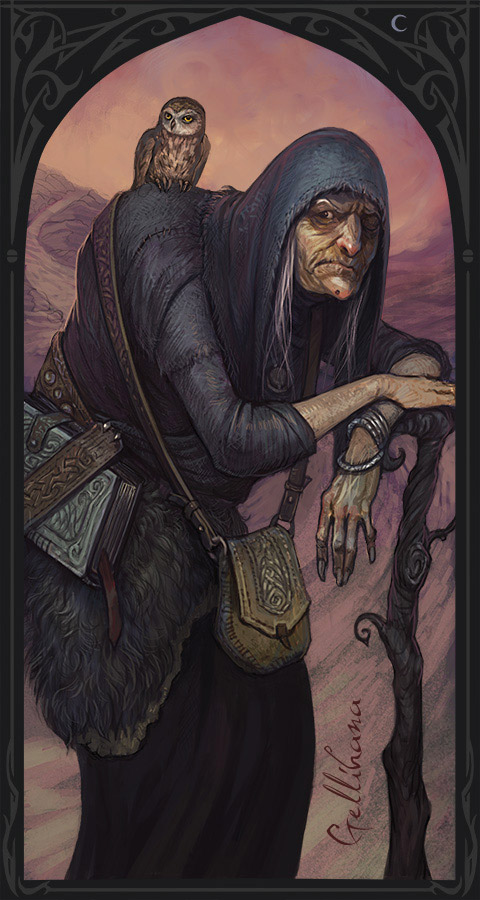
\includegraphics[width=0.5\linewidth]{img/nevar.jpg}
\end{center}

\begin{monsterbox}{Nev\'{a}r}
	\begin{hangingpar}
		\textit{?? ??, Neutral ??}
	\end{hangingpar}
	\dndline%
	\basics[%
	armorclass = ??,
	hitpoints  = ??,
	speed      = ?? ft
	]
	\dndline%
	\stats[
	STR = \stat{}, % This stat command will autocomplete the modifier for you
	DEX = \stat{},
	CON = \stat{},
	INT = \stat{},
	WIS = \stat{},
	CHA = \stat{}
	]
	\dndline%
	\details[%
	% If you want to use commas in these sections, enclose the
	% description in braces.
	% I'm so sorry.
	languages = {Common},
	challenge = 20
	]
	\dndline%
	\monstersection{Description/Information}
	Nev\'{a}r is an old sorcerer. Not much is known about her. She is tall and frail (or at least appears so). It is impossible to tell anything about her from looking at her. This NPC is a wild card. It can be used with the story as seen fit (save the important things she contains to the campaign).
\end{monsterbox}

\begin{commentbox}{The Ying-Yang}
	The Ying-Yang (Baba and Nev\'{a}r) plays an important part of this campaign. 
	
	Baba is a wizard that is interested in helping the party learn. She contains a vast library of knowledge and knows much about the Trinity stone legends and myths. She can assist the party in learning more. Similarly, she will insist the party is not ready if they claim they are seeking Athereu and if they insist they are will put the party through tests to confirm it. One test is to teleport the party to the halls of no end. Another would be to send them into Rem Silva after something that would help them on their journey. These challenges would be designed to assist them in their journey. 
	
	Nev\'{a}r is an old witch. She appears to contain vast knowledge of the trinity stone legends as well, but acts as if she knows nothing. She can assist the party in acquiring clues and items that will help find their way to their goal. Specifically, she contains a map of Aethereu (the inside) which appears as a blank piece of paper until entering Aethereu. This map is pivotal to easily navigating the chamber. Alternatively, she can contain clues regarding successful passage through The Pluvian Forest, along with Baba.
\end{commentbox}

\begin{commentbox}{Samilah}
	Samilah, which is a name derived from Samson and Delilah meaning ``shining night''. She can be placed into the campaign in many ways but serves as the mortal embodiment of the Celestials. Her main goal is to destroy the San'graal which is the only mortal weapon known to be able to destroy the Celestials. She can disguise herself as any other sentient being and has a necklace that will protect her from any harm. She is mentally disciplined so that her mind cannot be messed with and has nearly unlimited capabilities. After destroying the San'graal she will lead the Celestial army in the conquest of Orilla.
\end{commentbox}
